\documentclass[conference]{IEEEtran}
\usepackage{amsmath,amssymb,booktabs,graphicx,url}
\usepackage[hidelinks]{hyperref}
\title{Qwen3-ASR-1.7B: Architecture and a Reproducible Small-Sample Speech Recognition Study}
\author{\IEEEauthorblockN{Alaa Boghdady}\IEEEauthorblockA{Cellula AI Internship -- Week 8, Task 2\\Experimental evaluation with recorded Colab results}}
\begin{document}
\maketitle
\begin{abstract}
This report examines Qwen3-ASR-1.7B and documents an actual Google Colab inference experiment. Six LibriSpeech utterances were evaluated in clean and paired synthetic-noise conditions, then four VCTK speakers with documented English/Scottish accent labels were added. Sixteen inputs from ten speakers produced forty-eight timed trials. Overall normalized word error rate (WER) was 2.508\% and character error rate (CER) was 0.501\%. Aggregate real-time factor was 0.216 and peak PyTorch-allocated inference memory was 3.945 GiB. These observations establish that the assigned model executed successfully under the recorded environment. They do not establish population-level accuracy, accent parity, multilingual performance or general noise immunity. Accent comparisons are exploratory because each group contains only two speakers and different utterances.
\end{abstract}
\begin{IEEEkeywords}
automatic speech recognition, Qwen3-ASR, WER, CER, reproducibility, noise robustness
\end{IEEEkeywords}
\section{Introduction and Scope}
An ASR system must recover linguistic content from an acoustic signal while separating meaningful errors from presentation differences. Lowercase predictions can be perfectly intelligible even when an uppercase reference produces a large case-sensitive edit distance. An evaluation therefore needs both a declared normalization policy and preserved raw outputs.

The present study combines architecture inspection with a small, repeatable inference experiment. It asks three bounded questions: does the assigned checkpoint run; how do clean and paired noisy inputs differ; and what latency and memory are observed? It is an exploratory engineering exercise, not a reproduction of the developers' complete benchmark. The uploaded CSVs and environment record, rather than a screenshot alone, are the numerical evidence.

\section{Architecture and Recognition Pipeline}
The technical report describes an AuT encoder, a projector and a Qwen3-1.7B language decoder. Input features have 128 filterbank dimensions; eightfold downsampling yields 12.5-Hz audio representations. The 1.7B variant uses a roughly 300M-parameter audio encoder with hidden width 1024. Dynamic attention windows span 1--8 seconds. Training progresses through AuT pretraining, Omni pretraining, ASR supervised fine-tuning and GSPO reinforcement learning. The report gives approximately 40 million pseudo-labelled hours for AuT pretraining and 50,000 utterances for the final RL stage~\cite{qwenreport}.

The released configuration specifies 24 audio-encoder layers with 16 heads and FFN width 4096. Its text component has 28 layers, hidden width 2048, FFN width 6144, 16 attention heads, eight key/value heads and vocabulary size 151936~\cite{config}. These fields describe checkpoint structure, not a separate parameter-count measurement. The model's name should not be interpreted as an independently verified total including every encoder and projector parameter.

\begin{figure}[t]
\centering\small
\fbox{\begin{tabular}{c}16-kHz mono waveform\\$\downarrow$\\128-bin acoustic features $\rightarrow$ AuT encoder\\$\downarrow$\\Projector $\rightarrow$ Qwen3 causal decoder\\$\downarrow$\\Language label and transcription\end{tabular}}
\caption{Conceptual ASR information flow, redrawn from the reported components~\cite{qwenreport}. This is not a layer-by-layer implementation diagram.}
\label{fig:pipeline}
\end{figure}

The decoder conditions text generation on projected audio representations. A useful abstract formulation is
\begin{equation}
p_\theta(y\mid x)=\prod_{t=1}^{T}p_\theta(y_t\mid y_{<t},P(E(F(x)))),
\end{equation}
where $F$ extracts acoustic features, $E$ is the encoder and $P$ is the projector. Output text tokens are not one-to-one acoustic frames or words. Tokenization, therefore, is distinct from the word segmentation used for WER. The configuration provides audio boundary token IDs and a causal text model~\cite{config}; the public processor/backend manages the input formatting~\cite{toolkit}.

The official toolkit lists 30 supported languages, including Arabic and English, plus 22 Chinese dialects; it also provides offline and streaming interfaces~\cite{toolkit}. This experiment uses offline transcription only. A separate forced aligner is not loaded, and no word timestamps or diarization results are claimed.
\clearpage
\section{Experimental Setup and Implementation}
\subsection{Data and Controlled Perturbation}
The notebook selected the first qualifying 2--30-second utterance for each of six distinct speakers while scanning a streamed LibriSpeech test-clean subset~\cite{librispeech}. The resulting durations were 2.165, 3.285, 3.505, 7.835, 15.770 and 22.570 seconds. Selection was deterministic by scan order, not a random representative sample. The six original clips totalled 55.13 seconds.

Each clean clip received a paired additive-white-noise variant at 10 dB signal-to-noise ratio. A fixed seed of 42 controlled noise generation. For clean signal $s$ and random noise $n$, the scaled mixture was
\begin{equation}
\tilde{s}=s+\frac{\operatorname{RMS}(s)}{10^{10/20}\operatorname{RMS}(n)}n.
\end{equation}
Common peak scaling prevented clipping before PCM-16 writing. This perturbation changes acoustic conditions without introducing a new speaker, accent or reference transcript. The twelve paired inputs represent six underlying utterances, not twelve independent observations. Four additional VCTK recordings~\cite{vctk} added two speakers labelled English (Southern England) and two labelled Scottish (Fife and Perth), through the KTH-hosted representation~\cite{vctkrep}. One mic1 clip per speaker was used; their total duration was 15.348 seconds. Labels came from dataset metadata, not speaker-ID inference or independent linguistic assessment.

\subsection{Runtime and Model Loading}
The submitted environment records a Tesla T4 with 14.563 GiB visible device memory, Python 3.13.16, PyTorch 2.14.1+cu130, CUDA 13.0, Transformers 4.57.6 and \texttt{qwen-asr} 0.0.6. The checkpoint was \texttt{Qwen/Qwen3-ASR-1.7B}, revision \texttt{7278e1e70fe206f11671096ffdd38061171dd6e5}. Loading used the official \texttt{Qwen3ASRModel.from\_pretrained} interface~\cite{toolkit}, batch limit one, a 512-token generation cap and automatic language detection.

The recorded requested dtype was \texttt{torch.bfloat16}. This is a software-setting observation; native hardware execution precision was not profiled. A future portability check should record parameter dtypes and native BF16 capability explicitly, or repeat using FP16 when needed. The run's successful outputs do not justify assumptions about Tensor Core instruction selection.

Cold model loading took 85.648 seconds and peaked at 4.376 GiB allocated memory. These costs are separate from the transcription latencies. Installation and download costs are not included in warm inference times. The extension ran in a later Colab session, also recorded as Tesla T4; a complete second environment freeze was not exported, limiting strict cross-session timing comparisons.

\subsection{Timing and Evaluation Policy}
One warm-up was excluded. Every input then ran three times with CUDA synchronization around the transcription call. Waveform file reading preceded timing; internal feature processing and decoding remained inside it. Per-sample latency is the median of three trials. Every sample's three predicted transcripts were identical in the uploaded trials.

For reference words $N$, substitutions $S$, deletions $D$ and insertions $I$, the metrics are
\begin{equation}
\mathrm{WER}=\frac{S+D+I}{N},\qquad
\mathrm{CER}=\frac{d_{\mathrm{edit}}(r_c,h_c)}{|r_c|}.
\end{equation}
Here $r_c,h_c$ are character sequences and $d_{\mathrm{edit}}$ is Levenshtein distance. Corpus rates aggregate edit counts and reference lengths rather than averaging per-clip percentages. JiWER performs the alignment~\cite{jiwer}; an independent dynamic-programming implementation subsequently checked the uploaded per-sample WER and CER.

Normalization applies Unicode NFC, casefolding, punctuation/symbol replacement with spaces and whitespace collapse. It does not fold Arabic letters or remove diacritics. CER includes the remaining spaces. Both raw and normalized strings are retained so that presentation effects remain auditable. WER is an error rate, not a classification accuracy, and can exceed 100\% when insertions are numerous.

Real-time factor is $\mathrm{RTF}=t_{\mathrm{processing}}/t_{\mathrm{audio}}$. Aggregate RTF divides summed median processing times by summed audio durations. Peak memory refers to PyTorch-allocated memory in the loaded process, including weights; it is neither incremental activation memory nor complete device usage.

\begin{table}[t]
\caption{Observed normalized results; rates shown as percentages.}
\label{tab:summary}\centering\small
\begin{tabular}{lrrrr}\toprule
Condition & $n$ & WER & CER & RTF\\\midrule
Clean & 6 & 2.899 & 0.635 & 0.2076\\
10 dB noise & 6 & 2.899 & 0.508 & 0.2090\\
VCTK English & 2 & 0.000 & 0.000 & 0.2553\\
VCTK Scottish & 2 & 0.000 & 0.000 & 0.2791\\
Combined & 16 & 2.508 & 0.501 & 0.2156\\\bottomrule
\end{tabular}
\end{table}
\section{Results and Discussion}
\subsection{Accuracy and Error Examples}
Table~\ref{tab:summary} reports the actual uploaded results. Each LibriSpeech condition contained 138 normalized reference words and four word edits. The four VCTK clips added 43 reference words with zero normalized word or character errors, giving overall WER $8/319=2.508\%$. Twelve of sixteen inputs had zero normalized word error. Per-clip zero error does not establish universal recognition accuracy.

For speaker 5639, clean transcription substituted \emph{there} for \emph{they} and \emph{the} for \emph{their}. With noise, \emph{they} was recovered, but \emph{Toledans} changed to \emph{Toledoans}; the \emph{their/the} mismatch remained. Both variants consequently had two substitutions among 48 reference words (4.167\% WER), despite different error identities. Equal WER therefore does not imply identical transcripts or identical acoustic sensitivity.

For speaker 2094, the reference ended in \emph{door place}, while both predictions used \emph{doorplace}. Word alignment counted a substitution and deletion, producing $2/49=4.082\%$ WER, while character distance was only one missing space. This example illustrates a token-boundary effect rather than two necessarily independent phonetic failures. Reference conventions deserve inspection alongside numerical scores.

All twelve LibriSpeech raw per-sample WER values were 100\% because uppercase references were compared with cased, punctuated predictions without normalization. This is a formatting-sensitive score, not evidence of failed recognition. The normalized metrics better isolate lexical differences under the stated policy; neither score should be silently substituted for the other.

The slightly lower noisy CER does not demonstrate that noise improves ASR. Only six paired utterances were tested, and an individual spelling or token-boundary change can alter the aggregate. No significance test or confidence interval is claimed for this convenience sample.

\subsection{Latency and Memory}
Median per-file times ranged from 0.676 to 3.962 seconds. The median across all sixteen per-file medians was 0.980 seconds. The combined 125.608 seconds of audio required approximately 27.08 seconds of summed median processing time, giving RTF 0.2156 (about 4.64 audio-seconds per processing-second). This aggregate ratio is not streaming time-to-first-token or a concurrent-serving throughput benchmark.

\begin{figure}[t]
\centering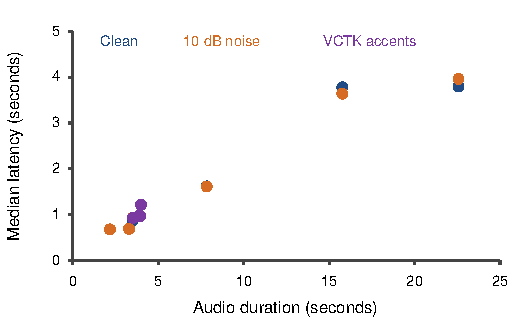
\includegraphics[width=\columnwidth]{latency.pdf}
\caption{Measured median transcription time versus input duration. Six LibriSpeech utterances have clean/noise pairs; four further points are VCTK clips. Nearby markers can overlap.}
\label{fig:latency}
\end{figure}

Peak allocated inference memory was 3.945 GiB. Longer inputs generally incurred greater latency in this sample, but duration alone does not determine decoding cost: output token count, kernels and runtime variation also matter. No batch-size sweep or alternative-backend comparison was run.

\subsection{Accent Coverage, Limitations and Improvements}
The evidence covers multiple speakers, durations, a controlled acoustic perturbation and two dataset-labelled accent groups. Zero errors on four short VCTK clips do not establish accent parity. It does \emph{not} cover real environmental noise, conversational speech, Arabic, streaming, very long audio or comparison with another ASR model. Developer-reported capabilities and benchmarks are not measured outcomes of this study. The official report's broader evaluations~\cite{qwenreport} cannot be transferred to this sixteen-input sample.

The VCTK inputs were packaged with reference text and provenance after the dataset-row service returned repeated HTTP 502/503 errors in Colab. Local-file inference then succeeded. Future work should balance utterances across accent groups, randomly sample more speakers, vary SNR and include a second ASR model. These improvements are proposals, not experiments already performed.

\section{Conclusion}
The assigned checkpoint successfully produced repeatable transcriptions in the submitted Colab run. Independent arithmetic checks support the uploaded error rates and median timings. The study shows low normalized error and sub-real-time processing for the tested inputs, with transparent scope and normalization effects. Documented English/Scottish accent coverage is included, while small sample sizes and separate execution sessions limit generalization.

\begin{thebibliography}{7}
\bibitem{qwenreport} Qwen Team, ``Qwen3-ASR technical report,'' arXiv:2601.21337, 2026. [Online]. Available: \url{https://arxiv.org/abs/2601.21337}
\bibitem{config} Qwen Team, ``Qwen3-ASR-1.7B configuration,'' Hugging Face. [Online]. Available: \url{https://huggingface.co/Qwen/Qwen3-ASR-1.7B/blob/main/config.json}
\bibitem{toolkit} Qwen Team, ``Qwen3-ASR: official inference toolkit,'' GitHub. [Online]. Available: \url{https://github.com/QwenLM/Qwen3-ASR}
\bibitem{librispeech} OpenSLR, ``LibriSpeech ASR dataset,'' Hugging Face, CC BY 4.0. [Online]. Available: \url{https://huggingface.co/datasets/openslr/librispeech_asr}
\bibitem{jiwer} Jitsi, ``JiWER: speech recognition evaluation,'' GitHub. [Online]. Available: \url{https://github.com/jitsi/jiwer}
\bibitem{vctk} J. Yamagishi, C. Veaux, and K. MacDonald, ``CSTR VCTK Corpus, version 0.92,'' University of Edinburgh, 2019, doi: 10.7488/ds/2645.
\bibitem{vctkrep} KTH Speech, Music and Hearing, ``VCTK dataset representation,'' Hugging Face, CC BY 4.0. [Online]. Available: \url{https://huggingface.co/datasets/kth-tmh/vctk}
\end{thebibliography}
\end{document}

